\section{Formación de pulsos, interferencia intersimbólica}

Supongamos que se envía por un canal de ancho $B<\infty$ una onda
PAM $\sum a_k p(t-kT_s)$, con pulsos rectangulares.

\begin{figure}[htb]
    \centering\begin{minipage}{\textwidth}
    \bpgf{Imagenes/formPuls/formPuls-1}
    \begin{blockdiagram}[xscale=0.8]
        \draw (-0.5,0) -- (0,0) node [anchor=north] {$0$}-- (0,1) -- (1,1) -- (1,0) node [anchor=north] {$T_s$} -- (2,0) -- (2,-1) -- (3,-1) -- (3,0) -- (3.5,0);
        \path (2,1) node {$x(t)$};
        \begin{scope}[shift={(7,0)}]
            \matrix[column sep=10mm]{
                \node[punto] (inicio) {}; & \node[block] (pasa) {PASABAJOS}; & \node[punto] (salida) {};\\
            };
            \draw [->] (inicio) -- (pasa);
            \draw [->] (pasa) -- (salida);
        \end{scope}
        \begin{scope}[shift={(11,0)}]
            \draw (-0.5,0) -- (0.25,0);
            \draw (0.25,0) .. controls (0.4,0.15) and (0.9, 0.7) .. (1,0.5);
            \draw (1,0.5) .. controls (1.1,0.25) and (1.6, -0.5) ..(1.5,-0.5);
            \draw (1.5,-0.5) .. controls (1.6,-0.6) and (2,-1) .. (2.3,-0.5);
            \draw (2.3,-0.5) .. controls (2.5,-0.25) and (3,0) .. (3.5,0);
            \path (2,1) node {$y(t)$};
        \end{scope}
    \end{blockdiagram}
    \endpgfgraphicnamed\end{minipage}
\end{figure}
\FloatBarrier

El detector debe basarse en la señal distorsionada para determinar el símbolo transmitido en cada instante de muestreo.

\paragraph{Problemas}
\begin{itemize}
    \item Los pulsos no llegan al máximo.
    \item Interferencia Intersimbólica (ISI): los pulsos se propagan a símbolos adyacentes.
\end{itemize}

\paragraph{Cualitativamente} podemos visualizar esto mediante el {\em diagrama de ojo.}
Supongamos por ejemplo pulsos polares, RZ, rectangulares
($p_{[0,T_s]}(t)$ y $-p_{[0,T_s]}(t)$). Sincronizo un osciloscopio
con $f_s$, observo la superposición de los pulsos.

\begin{figure}[htb]
    \centering
    \bpgf{Imagenes/formPuls/formPuls-2}
    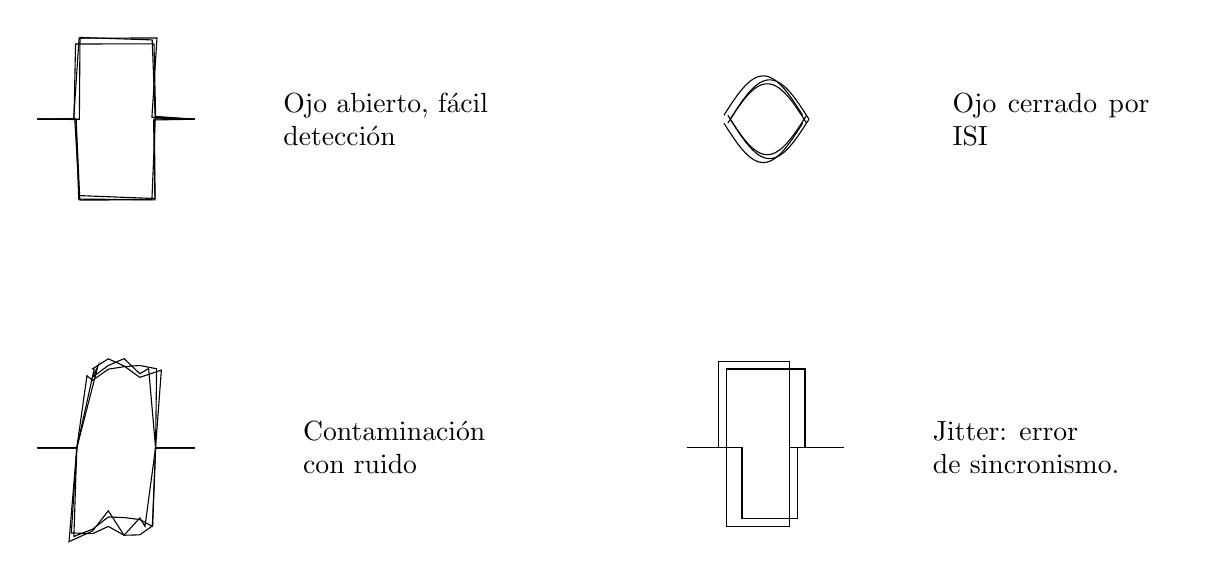
\begin{tikzpicture}
    \matrix[row sep=20mm, column sep=10mm]{
        \draw (-0.5,0) -- (0.05*rand,0.005*rand) -- (0.05*rand,1+0.05*rand) -- (1+0.05*rand,1+0.05*rand) -- (1+0.05*rand,0.05*rand) -- (1.5,0);
        \draw (-0.5,0) -- (0.05*rand,0.005*rand) -- (0.05*rand,1+0.05*rand) -- (1+0.05*rand,1+0.05*rand) -- (1+0.05*rand,0.05*rand) -- (1.5,0);
        \draw (-0.5,0) -- (0.05*rand,0.005*rand) -- (0.05*rand,1+0.05*rand) -- (1+0.05*rand,1+0.05*rand) -- (1+0.05*rand,0.05*rand) -- (1.5,0);
        \draw[yscale=-1] (-0.5,0) -- (0.05*rand,0.005*rand) -- (0.05*rand,1+0.05*rand) -- (1+0.05*rand,1+0.05*rand) -- (1+0.05*rand,0.05*rand) -- (1.5,0);
        \draw[yscale=-1] (-0.5,0) -- (0.05*rand,0.005*rand) -- (0.05*rand,1+0.05*rand) -- (1+0.05*rand,1+0.05*rand) -- (1+0.05*rand,0.05*rand) -- (1.5,0);
        \draw[yscale=-1] (-0.5,0) -- (0.05*rand,0.005*rand) -- (0.05*rand,1+0.05*rand) -- (1+0.05*rand,1+0.05*rand) -- (1+0.05*rand,0.05*rand) -- (1.5,0);
        & \path (0,0) node {\begin{minipage}{3cm}
        Ojo abierto, fácil \\detección\end{minipage}};
        & &
        \draw [domain=0:1, samples=50] plot ({\x+0.05},{0.5*sin(pi*\x r)});
        \draw [domain=0:1, samples=50] plot ({\x+0.02},{0.5*sin(pi*\x r)-0.05});
        \draw [domain=0:1, samples=50] plot ({\x-0.03},{0.5*sin(pi*\x r)+0.05});
        \draw [domain=0:1, samples=50,yscale=-1] plot ({\x+0.05},{0.5*sin(pi*\x r)});
        \draw [domain=0:1, samples=50,yscale=-1] plot ({\x+0.02},{0.5*sin(pi*\x r)-0.05});
        \draw [domain=0:1, samples=50,yscale=-1] plot ({\x-0.03},{0.5*sin(pi*\x r)+0.05});
        & \path (0,0) node {\begin{minipage}{2.5cm}
        Ojo cerrado por ISI\end{minipage}};\\

        \draw (-0.5,0) -- (0,0) -- (0+0.2*rand+0.1,1+0.2*rand) -- (0.2,1+0.2*rand) -- (0.4,1+0.2*rand) -- (0.6,1+0.2*rand) -- (0.8,1+0.2*rand) -- (1+0.2*rand-0.1,1+0.015*rand) -- (1,0) -- (1.5,0);
        \draw (-0.5,0) -- (0,0) -- (0+0.2*rand+0.1,1+0.2*rand) -- (0.2,1+0.2*rand) -- (0.4,1+0.2*rand) -- (0.6,1+0.2*rand) -- (0.8,1+0.2*rand) -- (1+0.2*rand-0.1,1+0.015*rand) -- (1,0) -- (1.5,0);
        \draw (-0.5,0) -- (0,0) -- (0+0.2*rand+0.1,1+0.2*rand) -- (0.2,1+0.2*rand) -- (0.4,1+0.2*rand) -- (0.6,1+0.2*rand) -- (0.8,1+0.2*rand) -- (1+0.2*rand-0.1,1+0.015*rand) -- (1,0) -- (1.5,0);
        \draw[yscale=-1] (-0.5,0) -- (0,0) -- (0+0.2*rand+0.1,1+0.2*rand) -- (0.2,1+0.2*rand) -- (0.4,1+0.2*rand) -- (0.6,1+0.2*rand) -- (0.8,1+0.2*rand) -- (1+0.2*rand-0.1,1+0.015*rand) -- (1,0) -- (1.5,0);
        \draw[yscale=-1] (-0.5,0) -- (0,0) -- (0+0.2*rand+0.1,1+0.2*rand) -- (0.2,1+0.2*rand) -- (0.4,1+0.2*rand) -- (0.6,1+0.2*rand) -- (0.8,1+0.2*rand) -- (1+0.2*rand-0.1,1+0.015*rand) -- (1,0) -- (1.5,0);
        \draw[yscale=-1] (-0.5,0) -- (0,0) -- (0+0.2*rand+0.1,1+0.2*rand) -- (0.2,1+0.2*rand) -- (0.4,1+0.2*rand) -- (0.6,1+0.2*rand) -- (0.8,1+0.2*rand) -- (1+0.2*rand-0.1,1+0.015*rand) -- (1,0) -- (1.5,0);
        & \path (0,0) node {\begin{minipage}{2.5cm}Contaminación con ruido\end{minipage}};
        & &
        \draw (-0.5,0) -- (0,0) -- (0,1) -- (1,1) -- (1,0) -- (1.5,0);
        \draw (-0.5,0) -- (-0.1,0) -- (-0.1,1.1) -- (0.8,1.1) -- (0.8,0) -- (1.5,0);
        \draw (-0.5,0) -- (0.2,0) -- (0.2,-0.9) -- (0.9,-0.9) -- (0.9,0) -- (1.5,0);
        \draw (-0.5,0) -- (0,0) -- (0,-1) -- (0.8,-1) -- (0.8,0) -- (1.5,0);
        & \path (0,0) node {\begin{minipage}{3cm}
        Jitter: error \\de sincronismo.\end{minipage}};\\
    };
    \end{tikzpicture}
    \endpgfgraphicnamed
\end{figure}
\FloatBarrier

\subsection*{¿Cómo analizar el problema cuantitativamente?}

Un primer enfoque sería estudiar el error $x(t)-y(t)$ en términos
de su potencia media
\[
\langle(x-y)^2\rangle = \int_{|f|>B} S_x(f)\d f.
\]
Si este error es pequeño en relación a $\langle x^2 \rangle$, es
probable que la detección funcione bien. Esto puede servir para
estimar a qué velocidad $f_s$ transmitir.

\begin{ejemplo} \mbox{}%$\phantom{1}$
\begin{center}\begin{minipage}{\textwidth}
    \bpgf{Imagenes/formPuls/formPuls-3}
    \begin{tikzpicture}
        \draw (-5,0) -- (5,0);
        \draw (0,-0.5) -- (0,5);
        \draw [samples=200,domain=-4.8:4.8] plot (\x,{4.5*(sin(2*\x r)/(2*\x))^2});
        \draw [samples=200,domain=-4.8:-pi,fill] plot (\x,{4.5*(sin(2*\x r)/(2*\x))^2});
        \draw [samples=200,domain=pi:4.8,fill] plot (\x,{4.5*(sin(2*\x r)/(2*\x))^2});
        \path (-pi,0) node [anchor=north] {$-2 f_s$} -- (-pi/2,0) node [anchor=north] {$-f_s$} -- (pi/2,0) node [anchor=north] {$f_s$} -- (pi,0) node [anchor=north] {$2 f_s$};
        \path (2,4) node {NRZ polar};
    \end{tikzpicture}
    \endpgfgraphicnamed\end{minipage}
\end{center}
Si señalilzamos a $f_s = \frac{B}{2}$, obtenemos
$\langle(x-y)^2\rangle = 5\%$ de $ \langle x^2\rangle$.
\end{ejemplo}

Sin embargo: para la detección digital, basada en muestrear la
salida en ciertos momentos, nos interesa el valor del error $x-y$
en los instantes de
   muestreo.  $\langle(x-y)^2\rangle$ me da un promedio en el tiempo que no es tan relevante. En
   particular, puedo aceptar una distorsión importante de los
   pulsos (y por tanto, un error medio grande), en la medida que no
   comprometa los instantes de detección. Estudiamos ese tema a continuación.

\subsection*{Problema de Nyquist}

Dado un canal de banda base, de ancho $B$, ¿cual es la máxima
velocidad de señalización $f_s$  a la que se puede transmitir una
onda PAM $\sum a_k p(t-kT_s)$,  permitiendo a la salida la
recuperación de los $\{a_k\}$ libre de errores? ¿Qué pulsos $p(t)$
alcanzan este máximo?

%\begin{remarksSN}
{\bf Notas:}
\begin{itemize}
        \item Aquí permitimos que los $\{a_k\}$ sean cualquier número real y deben recuperarse exactamente. En este sentido, se trata de una onda PAM analógica.
        Después particularizaremos a $\{a_k\}$ en un conjunto de símbolos $\mathcal{A}$.
        \item El problema es parecido (dual) al de muestreo, también estudiado por Nyquist. Allí buscábamos la mínima frecuencia de muestreo $f_m$ que permite reconstruir una señal $x(t)$ de banda $B$.
    \end{itemize}
%\end{remarksSN}

\paragraph{Respuesta:}
\begin{center}
    \col{f_s= 2B}
\end{center}

Para alcanzar este valor, elegimos el pulso (de Nyquist ideal)
$p(t)= \sinc (\pi f_s t)$:

\begin{center}\begin{minipage}{\textwidth}
    \bpgf{Imagenes/formPuls/formPuls-4}
    \begin{tikzpicture}
        \draw[->] (-5,0) -- (5,0) node [anchor=north] {$t$};
        \draw[->] (0,-1.5) -- (0,5) node [anchor=west] {$p(t)$};
        \path (0,4.5) node [anchor=east] {$1$};
        \draw [samples=200,domain=-4.8:4.8] plot (\x,{4.5*sin(2*\x r)/(2*\x)});
        \path (-pi,0) node [anchor=north east] {$-2 T_s$} -- (-pi/2,0) node [anchor=south east] {$-T_s$} -- (pi/2,0) node [anchor=south west] {$T_s$} -- (pi,0) node [anchor=north west] {$2 T_s$};
    \end{tikzpicture}
    \endpgfgraphicnamed

    \bpgf{Imagenes/formPuls/formPuls-5}
    \begin{tikzpicture}
        \draw[->] (-3,0) -- (3,0) node [anchor=north] {$f$};
        \draw[->] (0,-0.5) -- (0,2) node [anchor=west] {$\hat{P}(f)$};
        \draw (-2,0) node [anchor=north] {$-\frac{f_s}{2}$} -- (-2,1) -- (0,1) node [anchor=south west] {$T_s$} -- (2,1) -- (2,0) node [anchor=north] {$B=\frac{f_s}{2}$};
    \end{tikzpicture}
    \endpgfgraphicnamed\end{minipage}
\end{center}
El pulso tiene ancho de banda $B$, y por lo tanto la señal $x(t)$
pasa sin distorsión por el canal. Se recibe entonces la onda PAM
\[y(t)=x(t)=\sum_k a_k \sinc \left(\pi f_s (t-kT_s)\right).\]
Como el $\sinc$ es cero en todos los múltiplos de $T_s$ salvo
uno, se deduce que
\[y(k_0 T_s) = \sum_k a_k \sinc\left(\pi f_s (k_0-k)T_s\right) = a_{k_0}.\]
Entonces el muestreo de $y(t)$ recupera los símbolos.

Falta ver que esa velocidad de señalización no se puede superar.
Supongamos en cambio que tomo $f_s > 2B$. Consideremos el mensaje
$\{a_k\} = \ldots \quad 1 \quad 0 \quad 1 \quad 0 \quad 1\quad 0
\quad 1\quad \ldots$. \\
Para ese mensaje $x(t)$ es periódica, de período $2T_s$,
frecuencia fundamental $\frac{f_s}{2} > B$. Escribimos su serie de
Fourier  $x(t) = \sum_n \hat{X}_n\e^{jnf_s\pi t}$. En un canal
pasabajos ideal de ancho de banda $B$, se filtran todos los
armónicos salvo la continua, por tanto se recibe $y(t) \equiv
\hat{X}_0$.

 Claramente, de la continua no puedo
extraer el mensaje. En particular, la salida sería igual para el
mensaje complementario (cambiar $1$ por $0$).

\paragraph{Resumen} Dado un canal de ancho $B$, la
máxima velocidad de señalización PAM que permite la detección sin
interferencia intersimbólica es $f_s=2B$. El máximo se obtiene con
pulsos de Nyquist ideales, $p(t)=\sinc (\pi f_s t)$.

\subsubsection*{Limitaciones del pulso ideal $p(t)=\sinc (\pi f_s t)$}

Un problema obvio es que el sinc es no causal, requiere empezar en
$-\infty$. En la practica se debe truncar y retardar $p(t)$ para
poder generar algo causal. Como el sinc cae a cero en forma
relativamente lenta (como $\frac{1}{t}$) el truncado no es fácil
de hacer.

Otro problema: supongamos que hay un error de sincronización y
muestreamos en $t=\varepsilon$ en lugar de $0$:

\begin{align*}
    x(\varepsilon)  & = \sum a_k \sinc (\pi f_s \varepsilon - k\pi)\\
            & = \sum a_k \frac{\sen(\pi f_s \varepsilon) (-1)^k}{\pi f_s\varepsilon -k\pi}\\
            & = \underbrace{a_0 \frac{\sen(\pi f_s \varepsilon)}{\pi f_s \varepsilon}}_{\approx a_0} + \underbrace{\sum_{k\neq 0} a_k (-1)^k \frac{\sen(\pi f_s \varepsilon)}{\pi f_s \varepsilon - k \pi}}_{\text{término de error}}
\end{align*}

Cómo los términos decaen en valor absoluto como $\frac{1}{k}$, y
$\sum \frac{1}{k}=\infty$, se puede acumular bastante error de
ISI, donde los símbolos $a_k$ con $k\neq 0$ afectan la detección
de $a_0$.

Interesaría entonces, elegir pulsos que mantuvieran en condiciones
ideales la ISI nula, pero que caigan más rápido a $0$ con $t$, o
sea que estén más concentrados en el tiempo. Naturalmente, esto
implica más ancho de banda.

Consideremos el pulso $p(t) = \sinc (\pi f_s t) m(t)$ donde
$m(0)=1$ y $m(t)$ varía ``lento''.

\begin{figure}[htb]
    \centering\begin{minipage}{\textwidth}
    \bpgf{Imagenes/formPuls/formPuls-6}
    \begin{tikzpicture}
        \draw [samples=200,domain=-5:5] plot (\x,{3*sin(5*\x r)/(5*\x)});
        \path (2,3) node {$\sinc (\pi f_s t)$};
        \begin{scope}[shift={(0,-3)}]
            \draw [samples=201, domain=-5:5] plot (\x,{cos(5*0.1*\x r)/(1-(5/pi*0.2*\x)^2)});
            \path (2,1.5) node {$m(t)$};
        \end{scope}
    \end{tikzpicture}
    \endpgfgraphicnamed\end{minipage}
\end{figure}
\FloatBarrier

Se cumplirá $p(0)=1$, $p(kT_s) = 0 \forall\,k\neq 0$, entonces de una sucesión $\sum a_k p(t-kT_s)$ se extraen los símbolos $a_k$ por muestreo.

\paragraph{¿Qué ancho de banda tiene ese pulso? Estudiamos la convolución:} \back

\begin{figure}[htb]
    \centering\begin{minipage}{\textwidth}
    \bpgf{Imagenes/formPuls/formPuls-7}
    \begin{tikzpicture}
        \path (-2.5,1) node {$\hat{P}(f)$};
        \draw [->] (-1.5,0) -- (1.5,0);
        \draw [->] (0,-0.5) -- (0,1);
        \draw (-1,0) node [anchor=north] {$-\frac{f_s}{2}$} -- (-1,0.5) -- (1,0.5) node [anchor=south west] {$T_s$} -- (1,0) node [anchor=north] {$\frac{f_s}{2}$};
        \path (2.5,0.5) node {\Huge$\ast$};
        \begin{scope}[shift={(7,0)}]
            \path (-2.5,1) node {$\hat{M}(f)$};
            \draw [->] (-1.5,0) -- (1.5,0);
            \draw [->] (0,-0.5) -- (0,1);
            \draw [samples=200,domain=-0.5:0.5] plot (\x,{1/4*(1+cos(pi*2*\x r))});
        \end{scope}
    \end{tikzpicture}
    \endpgfgraphicnamed\end{minipage}
\end{figure}
\FloatBarrier

\noindent Elegimos $\hat{M}(f)$ de banda limitada $\dfrac{\alpha
f_s}{2}$, $0<\alpha<1$ para que espectro total no crezca mucho.

\begin{figure}[htb]
    \centering\begin{minipage}{\textwidth}
    \bpgf{Imagenes/formPuls/formPuls-8}
    \begin{tikzpicture}
        \draw [->] (-7,0) -- (7,0);
        \draw [->] (0,-6.5) -- (0,2);
        \draw (-4,0) node [anchor=north] {$-\frac{f_s}{2}$} -- (-4,1) -- (0,1) node [anchor=south west] {$T_s$} -- (4,1) -- (4,0) node [anchor=north] {$\frac{f_s}{2}$};
        \begin{scope}[shift={(0,-2)}]
            \draw [->] (-7,0) -- (7,0) node [anchor=north] {$\sigma$};
            \draw [samples=200,domain=-1:1] plot (\x,{4/pi*cos(pi*\x/2 r)});
            \path (-1,0) node [anchor=north] {$-\alpha\frac{f_s}{2}$} -- (1,0) node [anchor=north] {$\alpha\frac{f_s}{2}$};
            \path (1,1) node {$\hat{M}$};
            \path (-1,0.5) node [anchor=east] {área $1$};
        \end{scope}
            \begin{scope}[shift={(0,-4)}]
            \draw [->] (-7,0) -- (7,0);
            \begin{scope}[shift={(-5,0)}]
                \draw [samples=200,domain=-1:1] plot (\x,{4/pi*cos(pi*\x/2 r)});
                \path (1,1) node [anchor=west] {$\hat{M}(f-\sigma)$};
                \path (0,0) node [anchor=north] {$f$};
            \end{scope}
        \end{scope}
        \begin{scope}[shift={(0,-6)}]
            \draw [->] (-7,0) -- (7,0) node [anchor=north] {$\sigma$};
            \draw [samples=200,domain=-5:-3] plot (\x,{1/2*(1+cos((\x-1)*pi/2 r))}) -- (3,1);
            \draw [samples=200,domain=3:5] plot (\x,{1/2*(1-cos((\x-1)*pi/2 r))});
            \path (-5,0) node [anchor=north] {$-\frac{f_s}{2}(1+\alpha)$} -- (5,0) node [anchor=north] {$\frac{f_s}{2}(1+\alpha)$};
            \draw[very thin] (-3,1) -- (-3,0) node [anchor=north] {$-\frac{f_s}{2}(1-\alpha)$};
            \draw[very thin] (3,1) -- (3,0) node [anchor=north] {$\frac{f_s}{2}(1-\alpha)$};
            \path (0,1) node [anchor=east] {$T_s$};
            \path (5,1) node {$\hat{P}(f)$};
        \end{scope}
        \draw [dotted] (4,0) -- (4,-6);
        \draw [dotted] (-4,0) -- (-4,-6);
    \end{tikzpicture}
    \endpgfgraphicnamed\end{minipage}
\end{figure}
\FloatBarrier

\begin{remarkSN} $\hat{P}(f)$ es de banda $\frac{f_s}{2}(1+\alpha)$. El parámetro $\alpha$ se llama ``exceso de ancho de banda''.
    $\hat{P}(f)$ es constante (igual a $T_s$) en la banda $|f|\leq \frac{f_s}{2}(1-\alpha)$.  $\hat{P}(\pm \frac{f_s}{2}) = \frac{T_s}{2}$, y $\hat{P}(f)$ baja en forma simétrica alrededor de ese punto.
    %su bajada alrededor del punto
%    $(\frac{T_s}{2},)$
%
%     La bajada de  tiene simetría respecto a ese
%    punto.
\end{remarkSN}


\begin{ejemplo}[Pulso de coseno alzado]
\begin{align*}
\hat{P}(f) & =
\begin{cases}
 T_s, & |f| \leq (1-\alpha) \frac{f_s}{2}  \\
 T_s \Big[\frac{1}{2} + \frac{1}{2} \cos\Big(\pi
\frac{|f|-(1-\alpha) \frac{f_s}{2} } {\alpha f_s} \Big)\Big], &
(1-\alpha) \frac{f_s}{2}  < |f| <
(1+\alpha) \frac{f_s}{2}  \\
0,&  |f| \geq (1+\alpha) \frac{ f_s}{2}
\end{cases}%\\
%p(t) & = \frac{\cos(\pi\alpha f_st)}{1-(2\alpha f_s t)^2} \
%\sinc(\pi f_s t)
\end{align*}
%  \[\frac{T_s}{2}\left\lbrace 1 \pm \cos\left[\left(f-\frac{f_s}{2}(1-\alpha)\right)\right]\right\rbrace\]
    Esto corresponde a $\hat{M}(f)=\frac{\alpha f_s}{2 \pi}\cos\left(\frac{\pi f}{\alpha
f_s}\right)\qquad \text{ con }f \in
\left[-\alpha\frac{f_s}{2},\alpha\frac{f_s}{2}\right]$.

    Ecuación en el tiempo:
    \begin{align*}
        m(t)    = \mathcal{F}^{-1}\left[\hat{M}(f)\right] = \frac{\cos(\pi \alpha f_s t)}{1-(2 f_s \alpha t)^2}
    \end{align*}
\[ \Rightarrow \col{p(t) = \frac{\cos(\pi \alpha f_s t)}{1-(2 f_s \alpha t)^2} \sinc (\pi f_s
t)}\] En particular $p(t)$ cae como $\frac{1}{t^3}$, mucho más
concentrado en el tiempo.
    \FloatBarrier
    \begin{figure}[htb]
        \centering\begin{minipage}{\textwidth}
        \bpgf{Imagenes/formPuls/formPuls-9}
        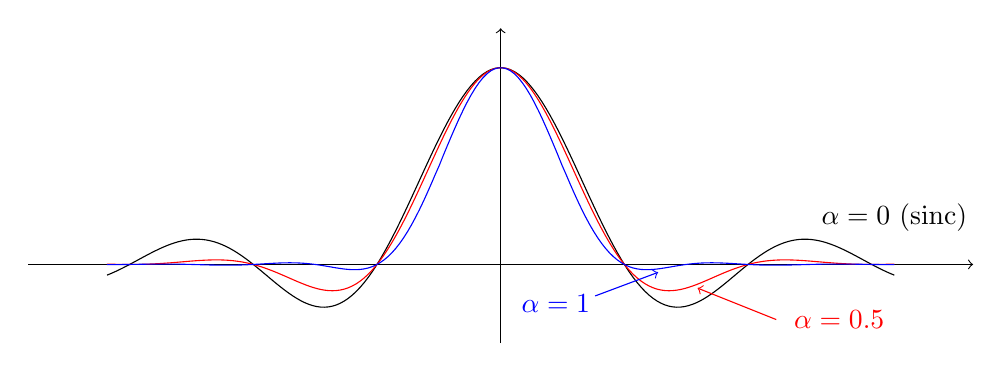
\begin{tikzpicture}
            \draw [->] (0,-1) -- (0,3);
            \draw [->] (-6,0) -- (6,0);
            \draw [samples=200,domain=-5:5] plot (\x, {2.5*sin(2*\x r)/(2*\x)});
            \draw [samples=200,domain=-5:5,red] plot (\x, {2.5*sin(2*\x r)/(2*\x)*cos(\x r)/(1-(2/pi*\x)^2)});
            \draw [samples=200,domain=-5:5,blue] plot (\x, {2.5*sin(2*\x r)/(2*\x)*cos(2*\x r)/(1-(4/pi*\x)^2)});
            \path (5,0.6) node {$\alpha=0$ (sinc)};
            \path (4.3,-.7) [red] node {$\alpha=0.5 $};
            \path [blue] (0.7,-0.5) node {$\alpha=1 $};
            \draw [->] [red] (3.5,-.7) -- (2.5,-0.3);
            \draw [->] [blue] (1.2,-0.4) -- (2,-0.1);
        \end{tikzpicture}
        \endpgfgraphicnamed\end{minipage}
    \end{figure}


\end{ejemplo}
\FloatBarrier

\subsection*{Otra forma de caracterizar los pulsos de Nyquist}

Imponemos que $p(t)$ cumpla $\begin{cases}
                                p(kT_s) = 0,& k\neq 0\\
                                p(0) = 1
                             \end{cases}$, $\hat{P}(f)$ de banda a lo sumo $2\cdot \frac{f_S}{2} = f_s$.

Estas dos condiciones se escriben como:
\begin{align*}
    p(t) \sum_{k=-\infty}^{+\infty} \delta(t-kT_s) &= \delta(t) \\
    \Leftrightarrow\hat{P}(f)\ast \frac{1}{T_s} \sum_{n=-\infty}^{+\infty} \delta(f-n f_s) &\equiv  1 \\
  \Leftrightarrow  \sum_{n=-\infty}^{+\infty} \hat{P}(f-n f_s) &\equiv
  T_s.
\end{align*}

\begin{minipage}{0.5\textwidth}
    \resizebox{\textwidth}{!}{
    \bpgf{Imagenes/formPuls/formPuls-10}
    \begin{tikzpicture}
        \draw [->] (-5,0) -- (5,0) node [anchor=north] {$f$};
        \draw [->] (0,-0.5) -- (0,1.5) node [anchor=west] {$\hat{P}$};
        \draw (2,0) .. controls (1,0) and (1,1) .. (0,1);
        \draw (-2,0) .. controls (-1,0) and (-1,1) .. (0,1);
        \draw [dotted] (0,0) .. controls (1,0) and (1,1) .. (2,1) .. controls (3,1) and (3,0) .. (4,0);
        \draw [dotted] (0,0) .. controls (-1,0) and (-1,1) .. (-2,1) .. controls (-3,1) and (-3,0) .. (-4,0);
        \path (-2,0) node [anchor=north] {$-f_s$};
        \draw [dashed] (1,1.2) -- (1,0) node [anchor=north] {$\frac{f_s}{2}$};
        \draw [dashed] (2,1.2) -- (2,0) node [anchor=north] {$f_s$};
    \end{tikzpicture}
    \endpgfgraphicnamed
    }
\end{minipage}
Sólo $2$ copias se superponen en $[0,f_s)$.

\begin{minipage}{0.3\textwidth}
    Que la suma sea constante $\Rightarrow$ simetría respecto a $\frac{f_s}{2}$
\end{minipage}
\begin{minipage}{0.5\textwidth}
    \resizebox{\textwidth}{!}{
    \bpgf{Imagenes/formPuls/formPuls-11}
    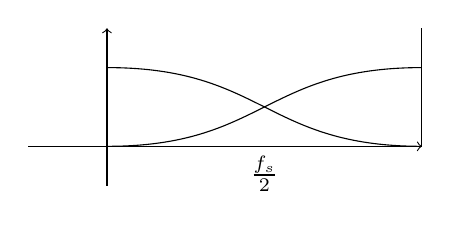
\begin{tikzpicture}[xscale=2]
        \draw [->] (-0.5,0) -- (2,0);
        \draw [->] (0,-0.5) -- (0,1.5);
        \draw (2,0) -- (2,1.5);
        \draw (2,0) .. controls (1,0) and (1,1) .. (0,1);
        \draw (0,0) .. controls (1,0) and (1,1) .. (2,1);
        \path (1,0) node [anchor=north] {$\frac{f_s}{2}$};
    \end{tikzpicture}
    \endpgfgraphicnamed
    }
\end{minipage}

\subsection*{Volvemos al tema de la eficiencia espectral}

\paragraph{Recordar}
    \begin{itemize}
        \item $f_s$: velocidad de señalización en Baudios
        ($\rfrac{\text{símb}}{\text{seg}}$).
        \item $vti = f_s \log_2 (M)$: velocidad de transmisión de información, bps.
        \item Eficiencia espectral: $\dfrac{vti}{B}$.
    \end{itemize}

   \noindent De acuerdo a Nyquist, la máxima eficiencia espectral que permite detección libre de ISI es
    \[\max_{f_s\leq 2B} \frac{f_s \log_2(M)}{B} = 2 \log_2 (M).\]

    \noindent Si en cambio, uso pulsos de Nyquist con exceso de ancho de banda $\alpha$, tenemos
    \[\frac{f_s}{2}(1+\alpha) = B \Rightarrow \text{ eficiencia espectral } \ \ \frac{2}{1+\alpha} \log_2 (M).\]

{\bf Nota:} Con $M$ arbitrario, en principio no hay límites a la
eficiencia espectral alcanzable. Sin embargo, para distinguir
símbolos en presencia de ruido, hay que separarlos (como se verá).
Agrandar $M$ implica entonces agrandar la amplitud de la señal y
por tanto la \emph{potencia}. Agrandar $vti$ para $B$ fijo tiene
un costo en potencia.
%
%
%        \begin{itemize}
%            \item Con
%            \item Sin
%        \end{itemize}
%%    \end{remarkSN}

\subsection*{Ecualización}

En diversas situaciones la interferencia intersimbólica no se
logra evitar, y se recibe una onda $x_R(t) = \sum a_k
\tilde{p}(t-kT_s)$ donde el pulso $\tilde{p}(t)$ tiene ISI.

\begin{figure}[htb]
    \centering\begin{minipage}{\textwidth}
    \bpgf{Imagenes/formPuls/formPuls-12}
    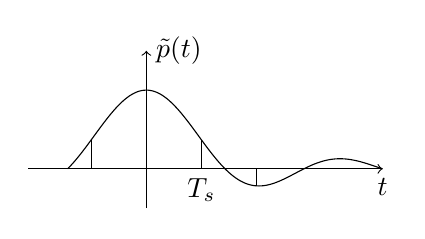
\begin{tikzpicture}
        \draw[->] (-1.5,0) -- (3,0) node [anchor=north] {$t$};
        \draw [->] (0,-0.5) -- (0,1.5) node [anchor=west] {$\tilde{p}(t)$};
        \draw [domain=-1:3,samples=200] plot (\x,{sin(pi*\x r)/(pi*\x)});
        \draw (0.7,{sin(pi*0.7 r)/(pi*0.7)}) -- (0.7,0) node [anchor=north] {$T_s$};
        \draw (-0.7,{sin(pi*(-0.7) r)/(-pi*0.7)}) -- (-0.7,0);
        \draw (1.4,{sin(pi*1.4 r)/(pi*1.4)}) -- (1.4,0);
    \end{tikzpicture}
    \endpgfgraphicnamed\end{minipage}
\end{figure}

Por ejemplo, se enviaron pulsos rectangulares por un canal muy
angosto. Una posible solución  en el receptor es compensar con un
\emph{filtro ecualizador} $\hat{H}_e$, que esencialmente invierte
el canal en la banda de interés. Una forma popular de hacerlo es
por un filtro transversal:

\begin{figure}[htb]
    \centering
    \resizebox{\textwidth}{!}{
    \bpgf{Imagenes/formPuls/formPuls-13}
    \begin{blockdiagram}
        \matrix[row sep=5 mm, column sep=10mm]{
            \node [etiqueta] (inicio) {$x_R(t)$}; & \node [punto] (p1) {}; & \node [block] (T1) {$T_s$}; & \node [punto] (p2) {}; & \node [block] (T2) {$T_s$}; & \node[punto] (p3) {}; & & \node [etiqueta]  {$\cdots$}; &  & \node [punto] (p4) {}; & \node [block] (T3) {$T_s$};\\
            & \node [multD] (m1) {$c_{-N}$}; & & \node[multD] (m2) {$c_{-N+1}$}; & & & &  & & & & \node [multD] (m3) {$c_{N}$};\\
            & & & \node [operator] (sum1) {$+$}; & & \node [operator] (sum2) {$+$}; & \node [punto] (p5) {};& &\node [etiqueta]  {$\cdots$}; & & \node [punto] (p6) {};&\node [operator] (sum3) {$+$}; & \node [etiqueta] (salida) {$y(t)$};\\
        };
        \draw (inicio) -- (p1);
        \draw [-stealth] (p1) -- (T1);
        \draw (T1) -- (p2);
        \draw [-stealth] (p2) -- (T2);
        \draw [-stealth] (T2) -- (p3);
        \draw [-stealth] (p4) -- (T3);
        \draw [-stealth] (p1) -- (m1);
        \draw [-stealth] (p2) -- (m2);
        \draw [-stealth] (T3) -|  (m3);
        \draw [-stealth] (m1) |- (sum1);
        \draw [-stealth] (m2) -- (sum1);
        \draw [-stealth] (sum1) -- (sum2);
        \draw [-stealth] (sum2) -- (p5);
        \draw [-stealth] (p6) -- (sum3);
        \draw [-stealth] (m3) -- (sum3);
        \draw [-stealth] (sum3) -- (salida);
    \end{blockdiagram}
    \endpgfgraphicnamed
}
\end{figure}
%\[
%\hat{H}(f) = \left (\sum_{k=-N}^N c_k \e^{-j2\pi f k
%%T_s}\right)\e^{-j2\pi f k N T_s}
%\]
\begin{align*} y(t+NT_s) = \sum_{n=-N}^N c_n {x}_R(t-nT_s) =\sum_{n=-N}^N
c_n \sum_k a_k \tilde{p}(t-(k+n)T_s) =\sum_k a_k\hat{p}(t - kT_s),%
%\\
%\text{donde }\hat{p}(t) =\sum_{n=-N}^N c_n \tilde{p}(t-nT_s)
%\Longrightarrow \mbox{ salida es una onda PAM con pulso
%$\hat{p}(t)$, retardada $NT_s$.}
\end{align*}%
donde $\hat{p}(t) =\sum_{n=-N}^N c_n \tilde{p}(t-nT_s)
\Longrightarrow y(t)$ es una onda PAM con pulso $\hat{p}(t)$,
retardada $NT_s$.

La idea es elegir los $\{c_n\}$ de modo de {\em forzar los ceros}
$\hat{p}(kT_s) = 0$ para $k\pm 1, \pm 2,\ldots,\pm N$. Esto se
denomina Zero Forcing Equalizer (ZFE), y  asegura que no hay ISI
con los $N$ símbolos adyacentes.  Estas condiciones,
conjuntamente con $\hat{p}(0)=1$, dan
 $2N+1$ ecuaciones para determinar las $2N+1$ ganancias $c_n$.
Como dato para ajustar el filtro debemos conocer
$\tilde{p}(kT_s)$, lo cual puede obtenerse de un experimento.
También hay versiones con ajuste adaptativo.
